\documentclass{beamer}
\usepackage{graphicx}
\usepackage{amsmath, amssymb}
\usepackage{fontspec}
\usepackage{subcaption}
\usepackage[english,ukrainian]{babel}
\setsansfont{CMU Sans Serif}
\setmainfont{CMU Serif}
\setmonofont{CMU Typewriter Text}

\usetheme{Madrid}
\usecolortheme{seagull}

\title{Метаевристичні алгоритми визначення оптимального розміщення вітрових турбін
на вітровій електростанції}
\author{Завалій Олександр Миколайович}
\institute{Науковий керівник: Хайдуров Владислав Володимирович}
\date{}


\begin{document}
\setbeamertemplate{footline}{}

    \begin{frame}
        \titlepage
    \end{frame}

    \begin{frame}
        \frametitle{ктуальнiсть застосування вiтроенергетичних установок i вiтрових турбiн в умовах сьогодення.}
        Паризька угода 2015 року визначила відновлювану енергетику ключовим фактором у боротьбі зі зміною клімату, 
        а вітроенергетику — головним джерелом чистої енергії. Однак ефективність вітрових електростанцій залежить від 
        розміщення турбін. Для цього потрібно враховувати турбулентність від інших турбін, розміщення на рельєфі, вітра, а також 
        який саме тип турбіни краще встановити саме на цій місцевості.

        Методи оптимізації включають генетичні алгоритми, моделювання Монте-Карло, рою частинок та алгоритми 
        мурашиних колоній. Впровадження різних діаметрів роторів і змінної висоти турбін дозволяє підвищити ефективність. 
        Інновації у розташуванні та технологіях критично важливі для майбутнього розвитку вітроенергетики.
    \end{frame}

    \begin{frame}
        \frametitle{Огляд вiтроенергетичних установок та технологiй вiтрових турбiн.}
        \framesubtitle{Класифiкацiя систем перетворення енергiї вiтру.}
        \begin{enumerate}
            \item Широка класифікація на основі осі вітрових турбін:
            \begin{itemize}
                \item Турбіна з горизонтальною віссю. Вісь обертання є горизонтальною, а лопаті аеротурбіни вертикальні. Направлення встановлюється до вітру.
                \item Турбіна з вертикальною віссю. Вісь обертання вертикальна. Вітрила або лопаті також можуть бути вертикальними.
            \end{itemize}
            \item Класифікація за розміром:
            \begin{itemize}
                \item Малі турбіни (потужністю до 2 кВт). Використовуються в системах малої потужності.
                \item Турбіни середнього розміру (2–100 кВт).
                \item Великомасштабні або великогабаритні турбіни (100 кВт і більше). Використовуються для генерації електроенергії та розподілу в центральних електромережах.
            \end{itemize}
            \item Класифікація за типом вихідної потужності:
            \begin{itemize}
                \item Вихід постійного струму.
                \item Вихід змінного струму.
            \end{itemize}
        \end{enumerate}
    \end{frame}

    \begin{frame}
        \frametitle{Огляд технологiй вiтрових турбiн.}
        Технології вітрових турбін можна розділити на дві групи: вітрові турбіни з фіксованою швидкістю (FSWT) та вітрові турбіни зі змінною швидкістю (VSWT). 
        Завдяки швидким інноваціям і розробкам силової електроніки за останні роки відбулося величезне вдосконалення вітроенергетичних технологій. 
        Це призвело до заміни FSWT на VSWT. Нижче наведено деякі з особливостей обох технологій вітрових турбін.
    \end{frame}

    \begin{frame}
        \frametitle{Клас вітрових турбін з фіксованою швидкістю (FSWT).}
        \begin{itemize}
            \item Мають обмежений діапазон потужності, оскільки він працює з використанням фіксованої швидкості. 
            \item Не мають можливості регулювання напруги та частоти. 
            \item Мають міцну конструкцію, низькі експлуатаційні витрати, не потребують технічного обслуговування та прості у використанні.
            \item Потребують великої компенсації реактивної потужності під час перехідного стану, щоб відновити потік повітряного зазору. 
            \item Є дорогим через встановлення зовнішніх пристроїв компенсації реактивної потужності, таких як гнучкі системи передачі змінного струму, 
            які можуть бути статичними синхронними компенсаторами або енергетичними конденсаторами. 
            Також потрібна надпровідна система зберігання магнітної енергії для забезпечення реактивної потужності.
        \end{itemize}
    \end{frame}

    \begin{frame}
        \frametitle{Клас вітрових турбін зі змінною швидкістю (VSWT)}
        \begin{itemize}
            \item Мають високу ефективність перетворення енергії під час слабких та сильних вітрів, оскільки працюють зі змінною швидкістю.
            \item Мають менший акустичний шум і механічні навантаження.
            \item Мають кращу "якість" електроенергії в електромережах, не використовуючи зовнішніх компенсаторів реактивної потужності.
            \item Використовують перетворювачі потужності для вторинного збудження, від 20 до 30\% для системи DFIG і 100\% для системи PMSG.
            \item Мають нижчу вартість експлуатації, оскільки генерують електроенергію в мережу та допомагають забезпечити підтримку реактивної потужності для стабільності мережі.
        \end{itemize}
    \end{frame}
    
    \begin{frame}
        \frametitle{Схеми турбін зі змінною швидкістю}
        \begin{figure}[h!]
            \centering
            \begin{subfigure}[t]{0.2\textwidth}
                \centering
                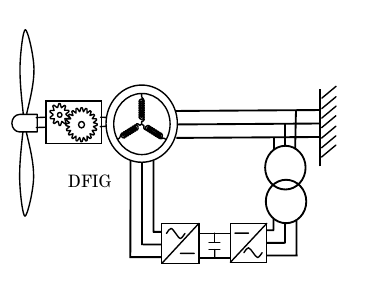
\includegraphics[width=\textwidth]{Pictures/FSIGWT.png}
                \caption{}
            \end{subfigure}
            \hfill
            \begin{subfigure}[t]{0.2\textwidth}
                \centering
                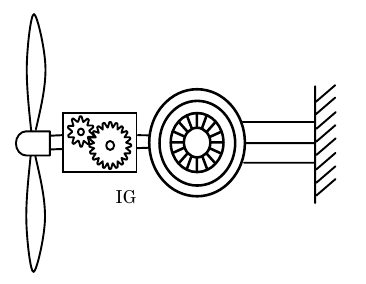
\includegraphics[width=\textwidth]{Pictures/DFIGVSWT.png}
                \caption{}
            \end{subfigure}
    
            \vskip\baselineskip
            \begin{subfigure}[t]{0.3\textwidth}
                \centering
                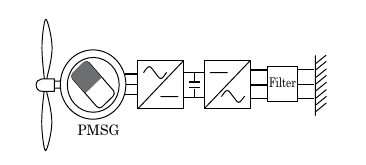
\includegraphics[width=\textwidth]{Pictures/PMSGVSWT.png}
                \caption{}
            \end{subfigure}
    
            \caption{(a) вітрова турбіна асинхронного генератора з фіксованою швидкістю, (b) вітрова турбіна змінної швидкості індукційного генератора з подвійним живленням, (c) вітрова турбіна змінної швидкості синхронного генератора з постійним магнітом.}
        \end{figure}
    \end{frame}

    \begin{frame}
        \frametitle{Математична модель оптимального розміщення вітрових турбін на електростанціях.}
        \framesubtitle{Wake Model}
        Термін «кільватерний слід» походить від сліду за кораблем. Як і кораблі, вітряні турбіни також створюють хвилі. Для вітряних турбін хвильовий ефект пов’язаний із дефіцитом швидкості 
        вітру та зменшенням вмісту енергії після виходу з вітрової турбіни. Отримуючи енергію з вітру, вітряна турбіна утворює уявний конус (шлях), який створює за собою повільніше та більш 
        турбулентне повітря. Базуючись на припущенні про збереження імпульсу в кільватері, 
        дефіцит швидкості на турбіні $i(vel\_ def_{ij})$, яка має відстань $x_{i,j}$ від турбіни $j$, можна обчислити за рівнянням:
        $$vel\_ def_{ij}=1-\dfrac{u}{u_0}=\dfrac{2a}{(1+\propto\frac{x_{i,j}}{r_r})^2}$$
        де $u_0$(м/с) – швидкість вітру, $x_{i,j}$(м) – відстань за потоком від вітрової турбіни, 
        $u$ – швидкість вітру за потоком після відстані $x_{i,j}$, $r_r$(м) – радіус ротора, $a$ — коефіцієнт осьової індукції.
    \end{frame}

    \begin{frame}
        \begin{figure}[h!]
            \centering
            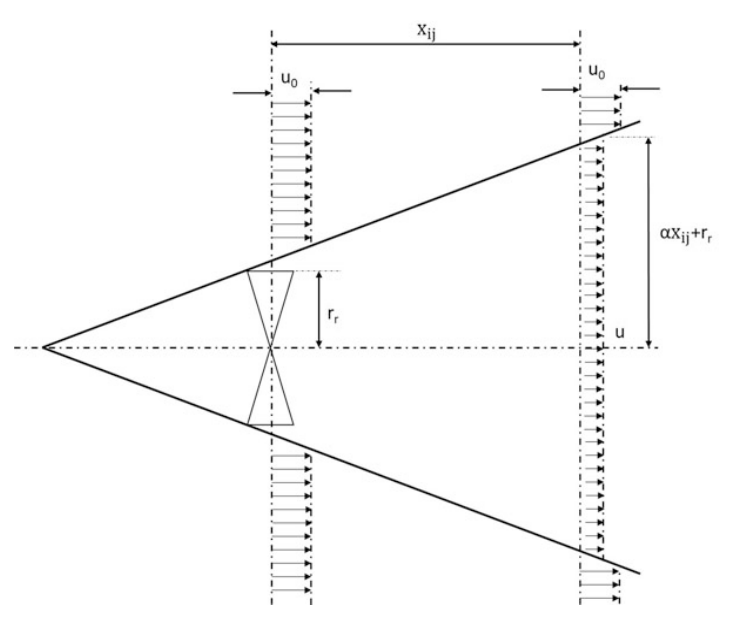
\includegraphics[width=0.75\textwidth]{Pictures/Wake model.png}
            \caption{Wake model}
        \end{figure}
    \end{frame}

    \begin{frame}
        \begin{figure}[h!]
            \centering
            \begin{subfigure}[t]{0.75\textwidth}
                \centering
                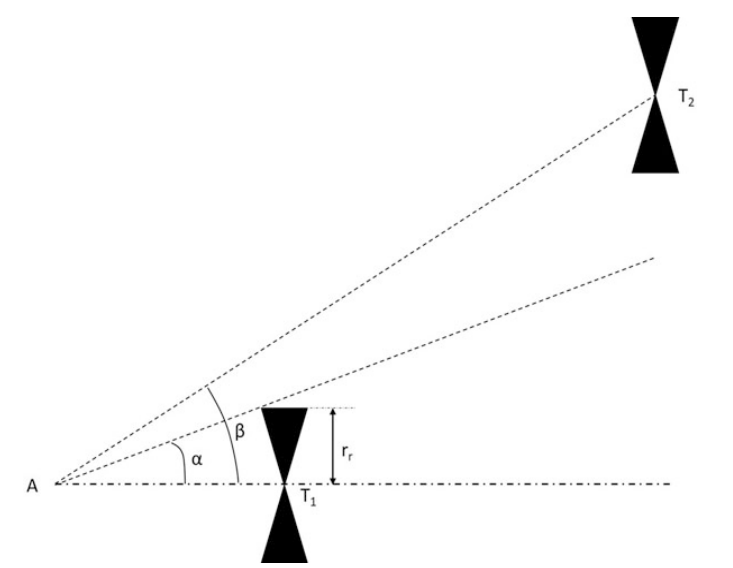
\includegraphics[width=\textwidth]{Pictures/Imaginary cone of a wind turbine.png}
            \end{subfigure}
            \caption{Уявний конус вітрової турбіни.}
            \label{fig:Imaginary_cone_wind_turbine}
        \end{figure}        
    \end{frame}

    \begin{frame}
        \frametitle{Power Model}
        Виробництво електроенергії, $P$(Вт), від однієї вітрової турбіни наведено в рівнянні:
        $$P=0.5\rho\pi r_r^2u^3C_p$$
        де $\rho$(кг/м3) - густина повітря, коефіцієнт потужності $C_p$ - це частка доступної потужності вітру, яку вловлює турбіна. 
        Це відображає ефективність перетворення потужності турбіни, яка в цій ситуації становить 42\%. Загальна потужність, вироблена на вітряній електростанції, 
        є сумою потужностей окремих турбін. Коли вітер протікає через турбіну, об’єм повітря, що надходить від турбіни має нижчу швидкість вітру та більшу турбулентність
        в порівнянні з вітром у вільному потоці. Таким чином, кожна з турбін може бути піддана впливу різної швидкості вітру, спричиненого хвилями.
    \end{frame}

    \begin{frame}
        Потужність розраховується за допомогою швидкості вільного потоку $u$, як рівняння:
        $$P(u)=
            \begin{cases} 
            0kW,\: u<3.5\\
            0.73u^3kW,\: 3.5\leqslant u<13 \\
            850kW,\: 13\leqslant 0<20 \\
            0,\: u\geqslant 20
            \end{cases}$$
        $$P_{tot}=\sum\limits^{N}_{i}P_i$$
        де $N$ - загальна кількість вітрових турбін. А цільова функція це
        $$\max\sum\limits^{N}_{i}P_i$$        
    \end{frame}

    \begin{frame}
        \frametitle{Висновки}
        Сучасний стан дослiджень у галузi вiтроенергетики демонструє значний прогрес у розвитку технологiй вiтрових турбiн та оптимiзацiї їх роботи. Основнi напрями включають
        вдосконалення конструкцiй турбiн, пiдвищення їх ефективностi та стiйкостi, впровадження нових матерiалiв i систем контролю.

        Водночас iснує низка проблем. Серед них є обмеження практичного впровадження
        нових моделей у рiзних клiматичних та географiчних умовах, необхiднiсть зниження витрат на виробництво й обслуговування турбiн, а також розв’язання проблем екологiчного впливу.

        Перспективи розвитку галузi полягають у подальшому вдосконаленнi алгоритмiв оптимiзацiї розташування турбiн, використаннi штучного iнтелекту для прогнозування ефективностi роботи установок, а також у бiльш глибокому аналiзi економiчної рентабельностi
        проєктiв. Вирiшення цих завдань сприятиме пiдвищенню частки вiтрової енергетики в
        загальному енергетичному балансi та забезпеченню сталого розвитку енергетики загалом.
    \end{frame}

\end{document}